% !TEX root = _main.tex


\begin{figure*}[tb]
	\centering
	\begin{minipage}{0.36\hsize}
		\centering
		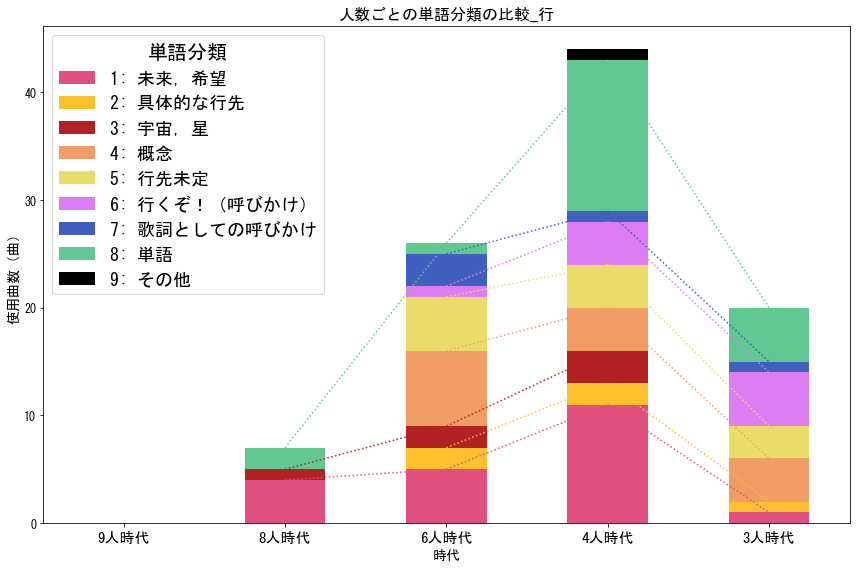
\includegraphics[width=\hsize]{fig/iku-ninzu.png}
		\caption{「行」人数時代別使用意味比較}
		\label{fig;iku-ninzu}
	\end{minipage}
	\begin{minipage}{0.62\hsize}
		\centering
		\captionof{table}{「行」人数別時代ごとの\kyokusu （()内は割合）}
		\label{tab:iku-uchi}
		\begin{tabular}{c|ccccc}
			\hline
			「行」の分類       & ８人時代     & ６人時代     & ４人時代      & ３人時代     & 合計        \\
			\hline\hline
			1:未来，希望      & 4 (57.1) & 5 (19.2) & 11 (25.0) & 1 (5.0)  & 21 (21.6) \\
			2:具体的な行先     & 0 (0.0)  & 2(7.7)   & 2 (4.5)   & 1 (5.0)  & 5 (5.2)   \\
			3:宇宙，星       & 1 (14.3) & 2 (7.7)  & 3 (6.8)   & 0 (0.0)  & 6 (6.2)   \\
			4:概念         & 0 (0.0)  & 7 (26.9) & 4 (9.1)   & 4 (20.0) & 15 (15.5) \\
			5:行先未定       & 0 (0.0)  & 5 (19.2) & 4 (9.1)   & 3 (15.0) & 12 (12.4) \\
			6:\scriptsize{行くぞ！（呼びかけ）} & 0 (0.0)  & 1 (3.8)  & 4 (9.1)   & 5 (25.0) & 10 (10.3) \\
			7:\scriptsize{歌詞としての呼びかけ} & 0 (0.0)  & 3 (11.5) & 1 (2.3)   & 1 (5.0)  & 5 (5.2)   \\
			8:単語         & 2 (28.6) & 1 (3.8)  & 14 (31.8) & 5 (25.0) & 22 (22.7) \\
			9:その他        & 0 (0.0)  & 0 (0.0)  & 1 (2.3)   & 0 (0.0)  & 1 (1.0)   \\
			\hline
			合計           & 7        & 26       & 44        & 20       & 97        \\
			\hline
		\end{tabular}
	\end{minipage}
\end{figure*}
